\documentclass[oneside,14pt]{extarticle}
\usepackage[utf8]{inputenc}
\usepackage[english,ukrainian]{babel}
\usepackage{amssymb,amsfonts,amsmath,amsthm,mathtext,textcomp}
%\usepackage{fontspec}
% \setmainfont[Mapping=tex-text]{Times New Roman}
\usepackage[includehead, headsep=0pt, footskip=0pt, top=2cm, bottom=2cm, left=2cm, right=1cm]{geometry}
\usepackage{indentfirst}
\setlength{\parindent}{1cm}
\usepackage[onehalfspacing]{setspace}
\usepackage[headings]{fancyhdr}\usepackage{hyperref}
\usepackage{etoolbox}
\usepackage{flafter}
\usepackage{listings}
\usepackage{graphicx}
\usepackage{float}
\usepackage[labelsep=period]{caption}
\lstset{
	basicstyle=\scriptsize,
	inputencoding=utf8,
	extendedchars=\true,
	showstringspaces=true
}
\usepackage{array}
\fancyhf{}
\renewcommand{\headrulewidth}{0pt}
\pagestyle{fancy}
\fancyfoot[R]{\thepage}
\lstset{breaklines=true,}
\graphicspath{ {./pictures} }

\lstset{
	language=c,
	tabsize=4,
	keepspaces,
	showstringspaces=false,
}
\graphicspath{ {./pictures} }
\setlength{\parindent}{4em}
\setlength\tabcolsep{5px}

\newcommand\subject{Комп'ютерна графіка}
\newcommand\lecturer{доцент кафедри ПЗ \\ Левус Є. В.}
\newcommand\teacher{доцент кафедри ПЗ \\ Левус Є. В.}
\newcommand\mygroup{ПЗ-32}
\newcommand\lab{1-4}
\newcommand\theme{}
\newcommand\purpose{}

\begin{document}
\begin{normalsize}
	\begin{titlepage}
		\thispagestyle{empty}
		\begin{center}
			\textbf{МІНІСТЕРСТВО ОСВІТИ І НАУКИ УКРАЇНИ\\
				НАЦІОНАЛЬНИЙ УНІВЕРСИТЕТ "ЛЬВІВСЬКА ПОЛІТЕХНІКА"}
		\end{center}
		\begin{flushright}
			\textbf{ІКНІ}\\
			Кафедра \textbf{ПЗ}
		\end{flushright}
		\vspace{70pt}
		\begin{center}
			\textbf{ЗВІТ}\\
			про виконання лабораторних робіт № \lab\\
			\textbf{з дисципліни}: <<\subject>>\\
			\textbf{варіант}:  індивідуальний №2
		\end{center}
		\vspace{50pt}
		\begin{flushright}
			
			\textbf{Лектор}:\\
			\lecturer\\
			\vspace{10pt}
			\textbf{Виконав}:\\
			
			студент групи \mygroup\\
			Коваленко Д.М.\\
			\vspace{10pt}
			\textbf{Прийняла}:\\
			
			\teacher\\
			
			\vspace{28pt}
			«\rule{1cm}{0.15mm}» \rule{1.5cm}{0.15mm} 2023 р.\\
			$\sum$ = \rule{1cm}{0.15mm}……………\\
			
		\end{flushright}
		\vspace{\fill}
		\begin{center}
			\textbf{Львів — 2023}
		\end{center}
	\end{titlepage}

	\tableofcontents
	\pagebreak
	
	\section{Завдання}
	\subsection{Індивідуальний варіант}
	\begin{enumerate}
		\item[1)] Побудувати фрактальні зображення: \begin{enumerate}
			\item[1.1)] Фрактал Мандельброта $f(z)=z\cdot z+c$. Можливість згенерувати різні
			зображення, а саме для: \begin{enumerate}
				\item[-] різних кольорових схем,
				\item[-] різного масштабування.
			\end{enumerate}
			\item[1.2)] Броунівський рух.
		\end{enumerate}
		\item[2)] Колірні моделі: RGB і HSV. Змінити насиченість по зеленому кольору.
		\item[3)] Реалізувати рух для паралелограма, введеного за його вершинами, на основі
		повороту за годинниковою стрілкою відносно вибраної вершини з одночасним його
		зменшення у А разів.
	\end{enumerate}

	\section{Теоретичні відомості}
	\subsection{Опис функцій програми}
	\subsubsection{Діаграма прецедентів програми}
	\begin{figure}[H]
		\centering
		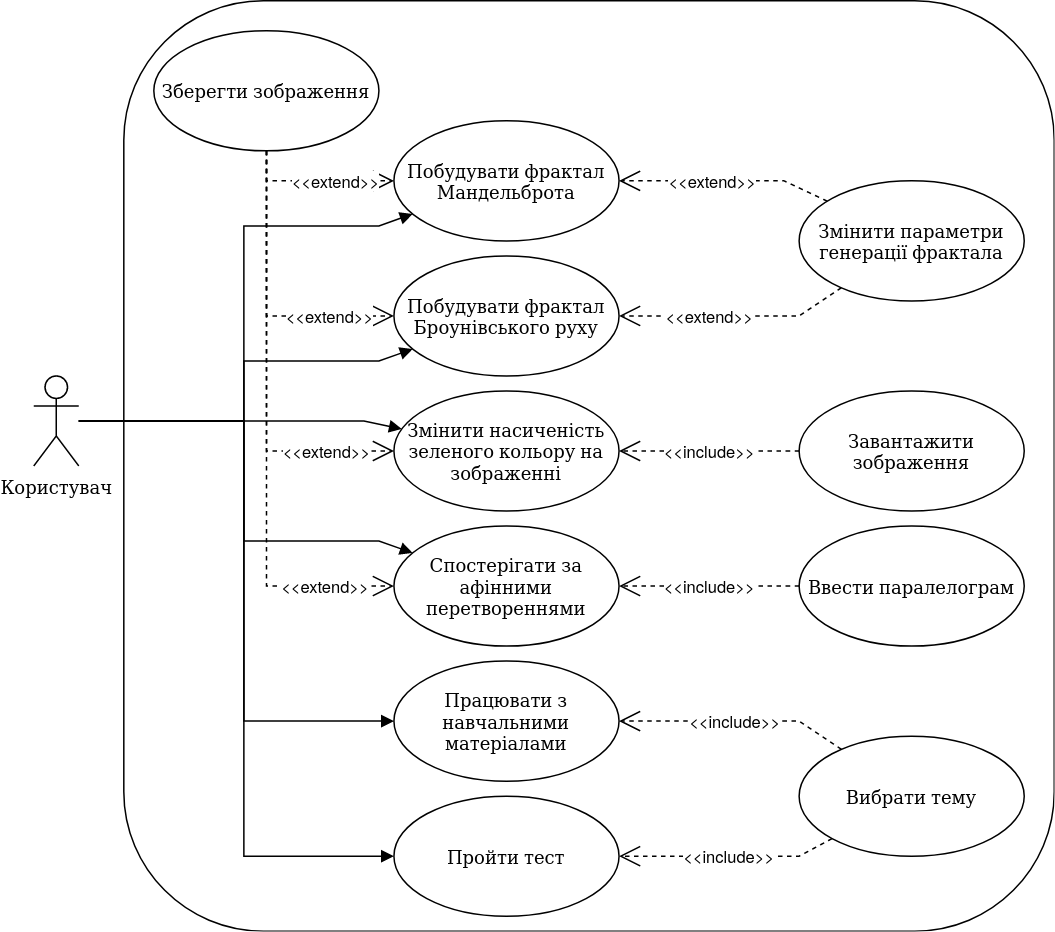
\includegraphics[scale=0.43]{d.drawio}
		\caption{Діаграма прецедентів програми}
	\end{figure}
	
	\subsubsection{Специфікація функцій програми}
	\begin{enumerate}
		\item Навчальні матеріали та інтерактивні елементи:
		Програма має вбудований розділ з навчальними матеріалами, які стосуються теми комп'ютерної графіки відповідно до варіанту.
		Використання інтерактивних елементів, таких як підказки, демонстрації, інтелектуальний помічник, опитувальник і ігрові елементи для покращення процесу навчання.
		\item Відповідні дії на неправильно введені дані:
		Реалізація обробки неправильно введених даних користувачем з метою попередження помилок та забезпечення зручного користувацького досвіду.
		Виведення інформативних повідомлень про помилки та надання користувачеві можливості внести корективи.
		\item Користувацькі інтерфейси:
		Створення UI-дизайну для шести виглядів системи (початковий екран, вікно для Л2, вікно для Л3, вікно для Л4, два вікна навчальних матеріалів) відповідно до методичних вказівок та з використанням інструментів Figma або Sketch.
		Забезпечення імплементації мокапів в програмній частині лабораторного практикуму.
		\item Інтерактивне навчання:
		Використання інтерактивних елементів для поліпшення процесу навчання, таких як динамічні підказки, демонстрації, опитування та ігровізація.
		Забезпечення можливості користувачам взаємодіяти з програмою, щоб активно освоювати матеріал.
		\item Звіт та презентація:
		Визначення характеристик системи, які дозволяють її вважати навчальною, та демонстрація цього під час захисту роботи.
		У звіті вказання результатів роботи, а також аналіз труднощів, які виникали під час виконання проекту.
		\item Інші функції:
		Забезпечення введення користувачем усіх параметрів для генерації фрактальних зображень, взаємодії з кольоровими схемами та рухомими зображеннями.
		Реалізація динамічної зміни відрізку координатної площини та збереження змін у графічному файлі.
	\end{enumerate}
	
	\subsection{Алгоритми фракталів}
	\subsubsection{Фрактал Мандельброта}
	\begin{enumerate}
		\item Визначте область комплексної площини, яку ви хочете відобразити (наприклад, $-2 \leq \text{Re}(z) \leq 2$ та $-2 \leq \text{Im}(z) \leq 2$).
		\item Розбийте цю область на пікселі.
		\item Для кожного пікселя $(x, y)$ визначте відповідну точку $c$ в комплексній площині, де $\text{Re}(c) = x$ та $\text{Im}(c) = y$.
		\item Визначте початкову точку $z$ як $z = 0$.
		\item Застосуйте ітераційну формулу $z_{n+1} = z_n^2 + c$ для обчислення наступних значень $z$.
		\item Повторюйте крок 5 до тих пір, поки $|z|$ не перевищить певне задане значення або до досягнення максимальної кількості ітерацій.
		\item Визначте колір пікселя відповідно до кількості ітерацій, яку знадобилось повторити для виходу з ліміту.
		\item Повторіть процес для кожного пікселя.
		\item Зобразіть отриманий зображення.
	\end{enumerate}
	
	\subsubsection{Броунівський рух}
	\begin{enumerate}
		\item Встановіть початкову точку $(x_0, y_0)$ у випадковому місці на площині.
		\item Для кожної ітерації $i$:
		\begin{enumerate}
			\item Згенеруйте два випадкових числа $\Delta x_i$ та $\Delta y_i$ з нормального розподілу.
			\item Оновіть координати: $x_i = x_{i-1} + \Delta x_i$ та $y_i = y_{i-1} + \Delta y_i$.
		\end{enumerate}
		\item Зобразіть отримані точки $(x_i, y_i)$ для всіх ітерацій на координатній площині.
	\end{enumerate}
	
	\subsection{Анотація кольорових моделей}
	\subsubsection{Модель RGB (Red, Green, Blue)}
	    Кольори визначаються комбінацією трьох основних кольорів: червоного (Red), зеленого (Green) і синього (Blue).
	Кожен канал може мати значення від 0 до 255, де 0 означає відсутність кольору, а 255 - максимальну інтенсивність кольору.
	
	\paragraph{Практичне застосування:}
	\begin{itemize}
		\item Використовується в комп'ютерних моніторах, телевізорах, фотографії та веб-дизайні.
		\item Кольорові простори, такі як sRGB, Adobe RGB, використовують RGB для представлення кольорів.
	\end{itemize}
	
	\paragraph{Переваги:}
	\begin{itemize}
		\item Просте обчислення та легке використання в графіці та програмуванні.
		\item Ідеально підходить для електронних пристроїв, які використовують світлодіоди для відображення кольорів.
	\end{itemize}
	
	\paragraph{Недоліки:}
	\begin{itemize}
		\item Модель не завжди ефективно відображає сприйняття кольорів людьми.
		\item Перевага одного кольору може призвести до втрати інших важливих деталей.
	\end{itemize}
	
	\subsubsection{Модель HSV (Hue, Saturation, Value)}
	Модель кольорів HSV (Відтінок, Насиченість, Значення) представляє кожен колір за допомогою його відтінку, насиченості та яскравості, що дозволяє інтуїтивно керувати характеристиками кольору для кращого творчого контролю.
	
	\paragraph{Практичне застосування:}
	\begin{itemize}
		\item Використовується в графічних програмах для зміни відтінку, насиченості та яскравості окремих кольорів.
		\item Зручно використовувати при виборі кольору на палітрі.
	\end{itemize}
	
	\paragraph{Переваги:}
	\begin{itemize}
		\item Забезпечує інтуїтивний підхід до редагування кольорів.
		\item Дозволяє легко змінювати параметри кольору без втрати співвідношення між ними.
	\end{itemize}
	
	\paragraph{Недоліки:}
	\begin{itemize}
		\item Може виглядати складніше для програмування або використання в окремих алгоритмах порівняно з RGB.
		\item Іноді не так ефективна, як RGB, при взаємодії з певними видами апаратного обладнання.
	\end{itemize}
	
	\subsection{Оптимальний матричний вираз афінних перетворень}
	\textbf{Умова}: \textit{поворот, з одночасним масштабування навколо вказаної точки}.
	
	Нехай $[A(x, y), B(x, y),C(x, y), D(x, y)]$ - точки паралелограма, $R$ - кут повороту, $S$ - коефіцієнт масштабування, і $C(x, y)$ - центр повороту, тоді:
	
	\[
	\begin{bmatrix} 
		A_x & A_y & 1 \\
		B_x & B_y & 1 \\
		C_x & C_y & 1 \\
		D_x & D_y & 1
	\end{bmatrix}
	\cdot
	\begin{bmatrix} 
		1 & 0 & 0 \\
		0 & 1 & 0 \\
		-C_x & -C_y & 1
	\end{bmatrix} 
	\cdot
	\begin{bmatrix} 
		 \cos(R) & -\sin(R) & 0 \\
		\sin(R) & \cos(R) & 0 \\
		0 & 0 & 1
	\end{bmatrix} 
	\cdot
	\begin{bmatrix} 
		S & 0 & 0 \\
		0 & S & 0 \\
		0 & 0 & 1
	\end{bmatrix}
	\cdot
	\begin{bmatrix} 
		1 & 0 & 0 \\
		0 & 1 & 0 \\
		C_x & C_y & 1
	\end{bmatrix} \]
	\subsection{Реалізація графічного режиму}
	Для реалізації графічного режиму у проекті обрано комбінацію JavaScript та фреймворку Vue.js. Вибір цієї технології обумовлений її гнучкістю, ефективністю та широким спектром можливостей для розробки динамічних та інтерактивних графічних інтерфейсів. Vue.js дозволяє створювати компоненти, які легко інтегруються у графічний інтерфейс, спрощуючи розробку та обслуговування.
	
	Vue.js дозволяє зручно налаштовувати графічні параметри через використання директив та змінних стану компонентів. За допомогою Vue.js можна динамічно змінювати роздільну здатність, кольорову гаму, а також інші параметри графічного відображення відповідно до вимог проекту.
	
	Використання бібліотеки Chart.js дозволило точно налаштовувати різноманітні аспекти графіків. Здійснюючи контроль над кольорами, стилями, легендами та іншими параметрами, створено візуально привабливі та інформативні графічні представлення даних. Це забезпечує не тільки зручне сприйняття інформації, але й гнучкість для відображення різних аспектів даних.
	
	У використанні Vue.js можна створювати реактивні компоненти для керування графічним виведенням. Розробка полотна графічного виведення може здійснюватися за допомогою вбудованих директив та методів Vue.js, що спрощує відображення графічних об'єктів на екрані.
	
	Використання Canvas API спрощувало створення графічного виведення. Створено інтерактивні полотна, на яких відображено графічні об'єкти. Це дозволило ефективно малювати та оновлювати графіку, використовуючи можливості Vue.js для реактивного оновлення елементів.
	
	Vue.js дозволяє легко створювати та управляти графічними примітивами. Використання компонентів Vue.js для представлення графічних об'єктів, таких як лінії, круги чи прямокутники, надає можливість легко маніпулювати ними, встановлюючи їх розміри, колір та інші атрибути.
	
	Використання бібліотек Math.js дозволило проводити розрахунки та операції з числами в складних формулах, що особливо корисно при роботі з математичними аспектами графіків. Bootstrap забезпечив стилізацію та адаптивність інтерфейсу, зробивши його зручним для користувачів на різних пристроях.
	
	Використання JavaScript та Vue.js для реалізації графічного режиму дозволяє створювати динамічні та ефективні візуальні інтерфейси, які відповідають потребам проекту.
	\section{Результати}
	\subsection{Wireflow}
	\begin{figure}[H]
		\centering
		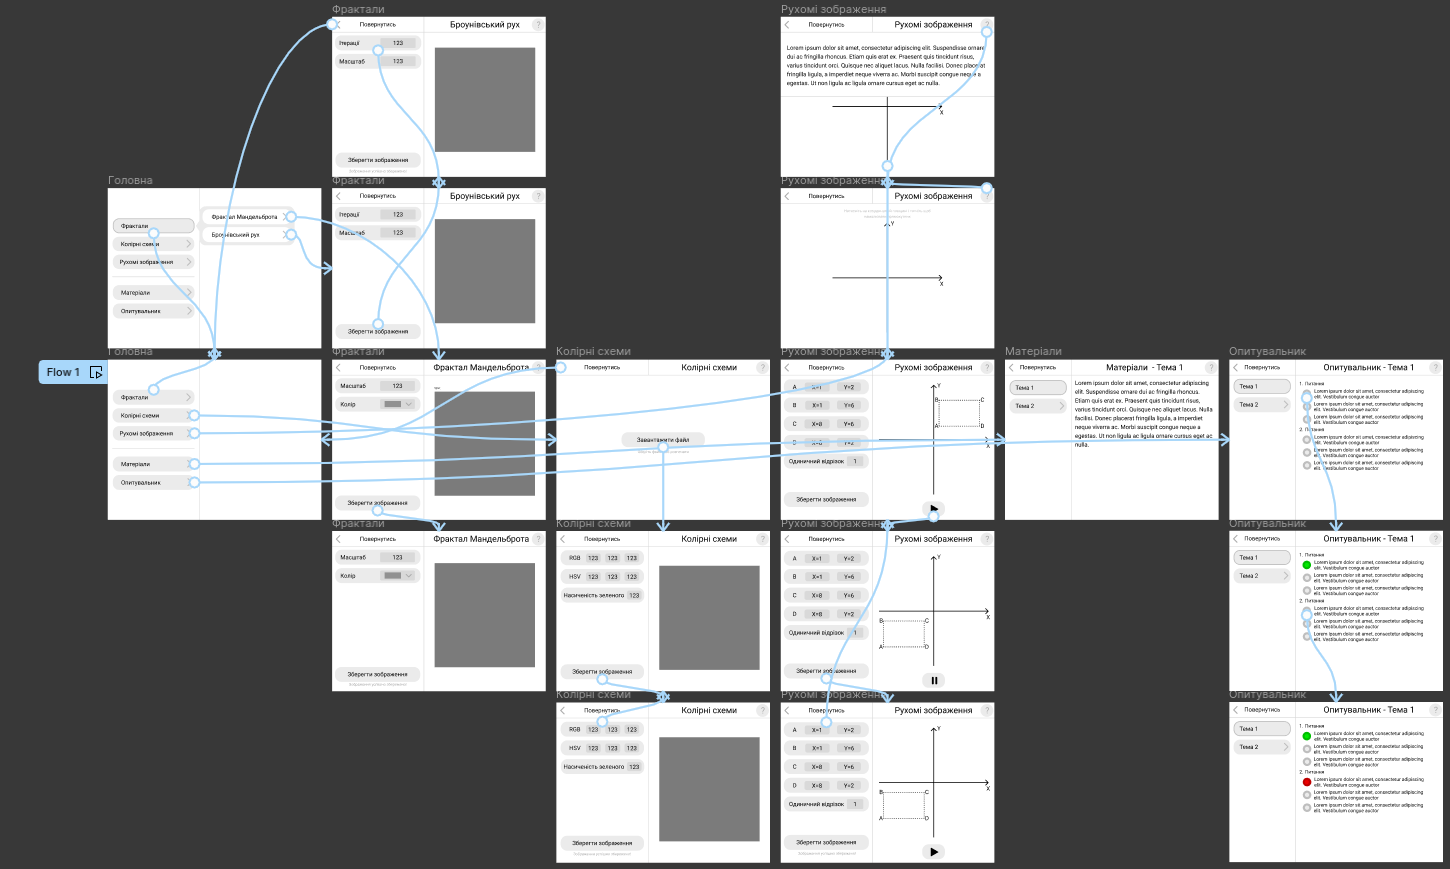
\includegraphics[scale=0.45]{wireflow}
		\caption{Wireflow виконаний у Figma}
	\end{figure}
	
	\subsection{Вигляд модулю <<Фрактали>>}
	\begin{figure}[H]
		\centering
		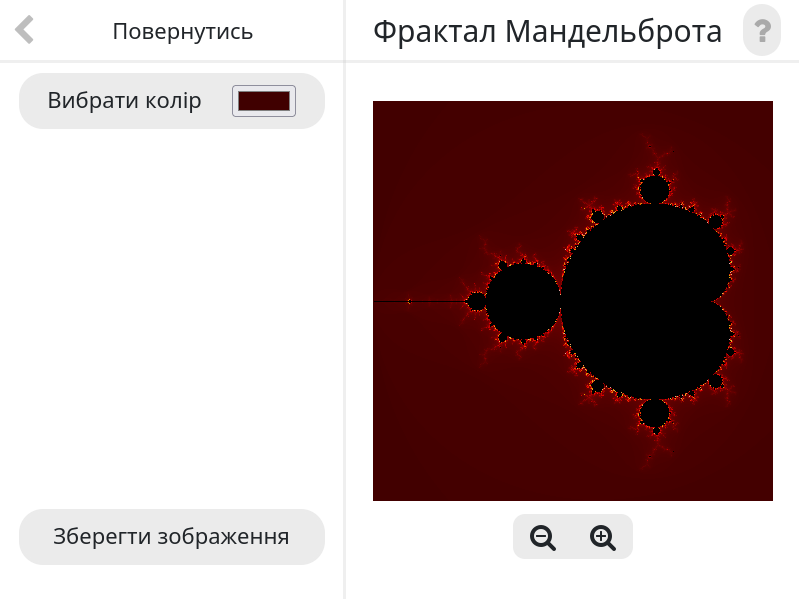
\includegraphics[scale=0.6]{11}
		\caption{Фрактал Мандельброта із виглядом за замовчуванням}
	\end{figure}
	
	\begin{figure}[H]
		\centering
		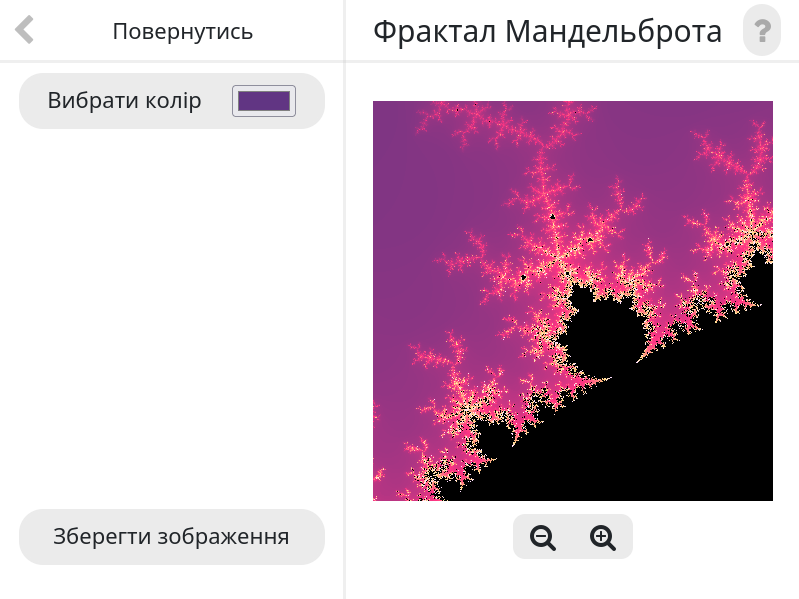
\includegraphics[scale=0.6]{12}
		\caption{Фрактал Мандельброта зі зміненим кольором та наближений}
	\end{figure}
	
	\begin{figure}[H]
		\centering
		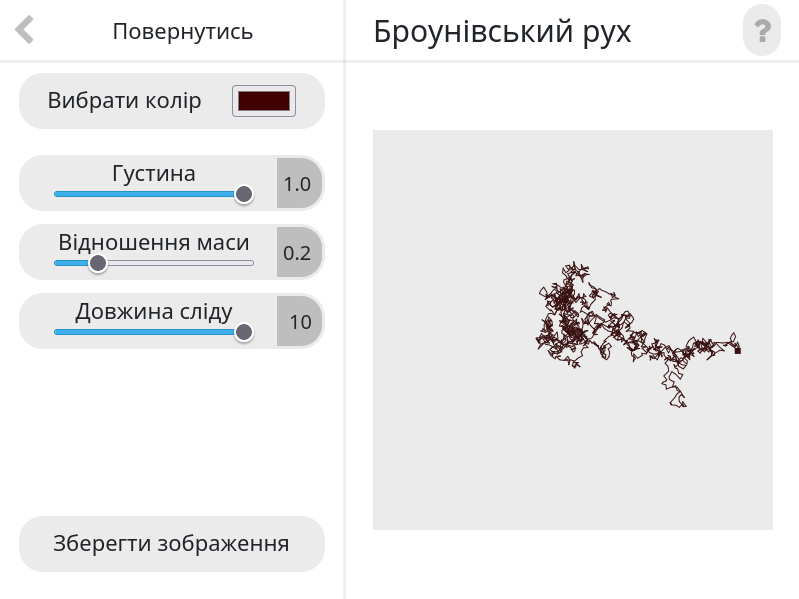
\includegraphics[scale=0.6]{21}
		\caption{Фрактал Броунівського руху}
	\end{figure}
	
	\subsection{Вигляд модулю <<Колірні схеми>>}
	\begin{figure}[H]
		\centering
		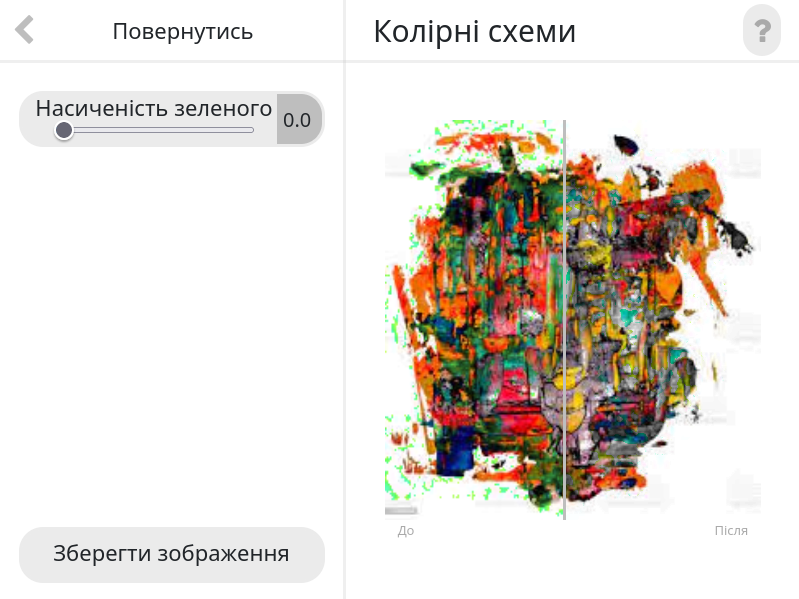
\includegraphics[scale=0.6]{31}
		\caption{Зміна насиченості зеленого кольору у зображення}
	\end{figure}
	
	\subsection{Вигляд модулю <<Рухомі зображення>>}
	\begin{figure}[H]
		\centering
		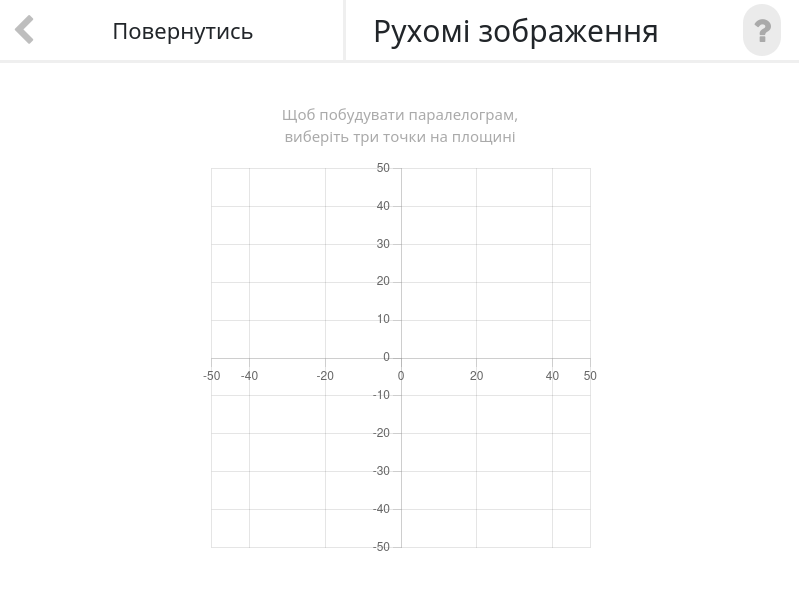
\includegraphics[scale=0.6]{41}
		\caption{Екран введення паралелограма}
	\end{figure}
	
	\begin{figure}[H]
		\centering
		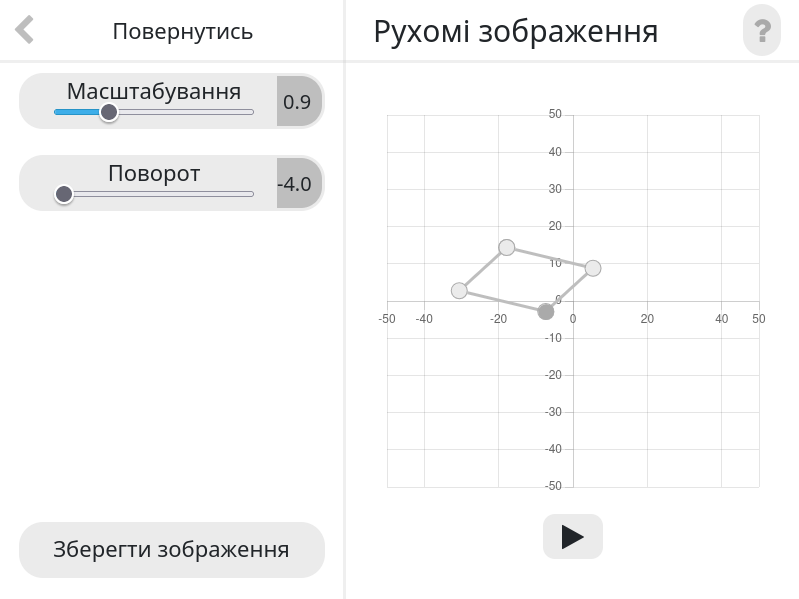
\includegraphics[scale=0.6]{42}
		\caption{Екран маніпуляції паралелограма}
	\end{figure}
	
	\subsection{Код програми}
	\paragraph{FractalsA.vue}
	:
	\begin{tiny}
		\begin{lstlisting}
<template>
<div class="d-flex" style="height: 540px; width: 800px;">
<div class="col" style="max-width: 343px;">
<div class="row d-flex justify-content-center">
<div class="btn btn-custom d-flex justify-content-center" style="margin-top: 13px;">
Вибрати колір
<input style="margin-left: 30px; margin-top: 3px;" type="color" value="#400000" name="" id="color" @change="generatePalette(); generateImage()">
</div>
</div>
<div class="row d-flex justify-content-center" style="margin-top: 367px;">
<div class="btn btn-custom" @click="saveImage">Зберегти зображення</div>
</div>
</div>
<div class="vr align-self-center" style="height: 100%; width: 3px; border: none; background-color: #bebebe;"></div>
<div class="col align-self-center">
<div class="row d-flex justify-content-center">
<div class="d-flex justify-content-center align-items-center" style="width: 400px; height: 400px;">
<canvas id="viewport" width="400" height="400" style="width: 400px; height: 400px; background-color: black;" @mousedown="onMouseDown"></canvas>
</div>
</div>
<div class="row d-flex justify-content-center">
<div class="btn btn-zoom btn-zoomout" @click="zoomOut">
<i class="fa fa-search-minus icon-zoomout"></i>
</div>
<div class="btn btn-zoom btn-zoomin" @click="zoomIn">
<i class="fa fa-search-plus icon-zoomin"></i>
</div>
</div>
</div>
</div>
</template>

<script>
export default {
	name: 'FractalsA',
	data() {
		return {
			canvasOffsetX: -200,
			canvasOffsetY: -200,
			shiftX: -100,
			shiftY: 0,
			zoom: 150,
			palette: [],
		};
	},
	computed: {
		canvas() {
			return document.getElementById('viewport');
		},
		context() {
			return this.canvas.getContext("2d");
		},
		image() {
			return this.context.createImageData(this.canvas.width, this.canvas.height);
		},
	},
	methods: {
		onMouseDown(event) {
			var pos = this.getMousePos(event);
			this.zoomFractal(pos.x, pos.y, 1, false);
			this.generateImage();
		},
		getMousePos(event) {
			var rect = this.canvas.getBoundingClientRect();
			return {
				x: Math.round((event.clientX - rect.left)/(rect.right - rect.left)*this.canvas.width),
				y: Math.round((event.clientY - rect.top)/(rect.bottom - rect.top)*this.canvas.height)
			};
		},
		zoomIn() {
			this.zoomFractal(200, 200, 2, true);
			this.generateImage();
		},
		zoomOut() {
			this.zoomFractal(200, 200, 2, false);
			this.generateImage();
		},
		zoomFractal(x, y, factor, zoomin) {
			if (zoomin) {
				this.zoom *= factor;
				this.shiftX = factor * (x + this.canvasOffsetX + this.shiftX);
				this.shiftY = factor * (y + this.canvasOffsetY + this.shiftY);
			} else {
				this.zoom /= factor;
				this.shiftX = (x + this.canvasOffsetX + this.shiftX) / factor;
				this.shiftY = (y + this.canvasOffsetY + this.shiftY) / factor;
			}
		},
		generateImage() {
			for (var y = 0; y < this.canvas.height; y++) {
				setTimeout(this.generateRow, 10, y);
			}
		},
		generateRow(y) {
			for (var x = 0; x < this.canvas.width; x++) {
				this.iter(x, y);
			}
		},
		iter(x, y) {
			var maxIter = 250;
			
			var zx = 0;
			var zy = 0;
			var cx = (x + this.canvasOffsetX + this.shiftX) / this.zoom;
			var cy = (y + this.canvasOffsetY + this.shiftY) / this.zoom;
			
			var i = 0;
			for (;zx * zx + zy * zy < 4 && i < maxIter; ++i) {
				const newZx = zx * zx - zy * zy + cx;
				const newZy = 2 * zx * zy + cy;
				
				zx = newZx;
				zy = newZy;
			}
			
			var index = Math.floor((i / (maxIter-1)) * 255);
			var color = this.palette[index] || { r:0, g:0, b:0};
			
			var pixelindex = (y * this.canvas.width + x) * 4;
			this.image.data[pixelindex] = color.r;
			this.image.data[pixelindex+1] = color.g;
			this.image.data[pixelindex+2] = color.b;
			this.image.data[pixelindex+3] = 255;
		},
		generatePalette() {
			var colorPicker = document.getElementById("color");
			var color = this.hexToRgb(colorPicker.value);
			var roffset = color.r;
			var goffset = color.g;
			var boffset = color.b;
			for (var i = 0; i < 256; i++) {
				this.palette[i] = { r:roffset, g:goffset, b:boffset};
				
				if (i < 85) {
					roffset += 2;
				} else if (i<170) {
					goffset += 2;
				} else if (i<255) {
					boffset += 2;
				}
			}
		},
		render() {
			window.requestAnimationFrame(this.render);
			this.context.putImageData(this.image, 0, 0);
		},
		saveImage() {
			var img = new Image();
			img.src = this.canvas.toDataURL('image/png');
			var downloadLink = document.createElement('a');
			downloadLink.href = img.src;
			downloadLink.download = 'mandelbrot.png';
			downloadLink.click();
			downloadLink.remove();
		},
		hexToRgb(hex) {
			hex = hex.replace(/^#/, '');
			
			var r = parseInt(hex.slice(0, 2), 16);
			var g = parseInt(hex.slice(2, 4), 16);
			var b = parseInt(hex.slice(4, 6), 16);
			
			return { r, g, b };
		}
	},
	mounted() {
		this.$emit('help', 'fractalsA');
		this.generatePalette();
		this.generateImage();
		this.render();
	},
};
</script>

<style scoped>
.btn-zoom {
	width: 60px;
	height: 45px;
	background-color: #ebebeb;
	border: 3px solid #ebebeb;
	border-radius: 0;
	margin-top: 13px;
}
.btn-zoomin {
	margin-right: auto;
	border-top-right-radius: 12px;
	border-bottom-right-radius: 12px;
}
.btn-zoomout {
	margin-left: auto;
	border-top-left-radius: 12px;
	border-bottom-left-radius: 12px;
}
.btn-zoom:active {
	background-color: #ebebeb;
	border: 3px solid #bebebe;
}
.icon-zoomin, .icon-zoomout {
	font-size: 28px;
}
.btn-custom {
	font-size: 22px;
	margin-bottom: 13px;
	border-radius: 24px;
	height: 56px;
	width: 306px;
	background-color: #ebebeb;
	border: 3px solid #ebebeb;
}
.btn:active {
	border: 3px solid #bebebe;
	background-color: #ebebeb;
}
</style>
		\end{lstlisting}
		\end{tiny}
		\paragraph{FractalsB.vue}
		:
		\begin{tiny}
		\begin{lstlisting}
<template>
<div class="d-flex" style="height: 540px; width: 800px;">
<div class="col" style="max-width: 343px;">
<div class="row d-flex flex-column align-items-center">
<div class="btn btn-custom d-flex justify-content-center" style="margin-top: 13px;">
Вибрати колір
<input style="margin-left: 30px; margin-top: 3px;" type="color" value="#400000" id="color" @change="update">
</div>
</div>
<div class="row d-flex justify-content-center" style="margin-top: 13px;">
<div class="btn-i btn-custom-i d-flex flex-column align-items-center" style="margin-top: 0px; position: relative;">
<span style="margin-top: -3px; margin-left: -35px;">Густина</span>
<input v-model="density" style="margin-top: -8px; margin-left: -35px; width: 200px;" type="range" id="density" min="0.01" max="1.0" step="0.01" value="0.2">
<span style="font-size: 20px; position: absolute; top: 50%; transform: translateY(-50%); right: 10px;">{{ parseFloat(density).toFixed(1) }}</span>
</div>
</div>
<div class="row d-flex justify-content-center">
<div class="btn-i btn-custom-i d-flex flex-column align-items-center" style="margin-top: 0px; position: relative;">
<span style="margin-top: -3px; margin-left: -35px;">Відношення маси</span>
<input v-model="massRatio" style="margin-top: -8px; margin-left: -35px; width: 200px;" type="range" id="mass-ratio"  min="0.01" max="1.01" step="0.01" value="0.2">
<span style="font-size: 20px; position: absolute; top: 50%; transform: translateY(-50%); right: 10px;">{{ parseFloat(massRatio).toFixed(1) }}</span>
</div>
</div>
<div class="row d-flex justify-content-center">
<div class="btn-i btn-custom-i d-flex flex-column align-items-center" style="margin-top: 0px; position: relative;">
<span style="margin-top: -3px; margin-left: -35px;">Довжина сліду</span>
<input v-model="traceLength" style="margin-top: -8px; margin-left: -35px; width: 200px;" id="traceLength" type="range" min="1" max="10001" step="10">
<span style="font-size: 20px; position: absolute; top: 50%; transform: translateY(-50%); right: 10px;">{{ parseFloat(traceLength / 1000).toFixed(0) }}</span>
</div>
</div>
<div class="row d-flex justify-content-center" style="margin-top: 154px;">
<div class="btn btn-custom" @click="saveImage">Зберегти зображення</div>
</div>
</div>
<div class="vr align-self-center" style="height: 100%; width: 3px; border: none; background-color: #bebebe;"></div>
<div class="col align-self-center">
<div class="row d-flex justify-content-center">
<div class="d-flex justify-content-center align-items-center" style="min-width: 400px; min-height: 400px;">
<canvas id="viewport" width="400" height="400" style="width: 400px; height: 400px; background-color: #ebebeb;" @mousedown="onMouseDown"></canvas>
</div>
</div>
</div>
</div>
</template>

<script>
export default {
	name: 'FractalsB',
	data() {
		return {
			color: "#370F0F",
			density: 1.0,
			massRatio: 0.2,
			traceLength: 10000,
			particle: {
				x: 200,
				y: 200,
				velocity: { dx: 0, dy: 0 }
			},
			traces: [],
		};
	},
	computed: {
		canvas() {
			return document.getElementById('viewport');
		},
		context() {
			return this.canvas.getContext("2d");
		},
		image() {
			return this.context.createImageData(this.canvas.width, this.canvas.height);
		},
	},
	methods: {
		update() {
			this.massRatio = document.getElementById('mass-ratio').value;
			this.density = document.getElementById('density').value;
			this.color = document.getElementById('color').value;
			this.traceLength = document.getElementById('traceLength').value;
			this.traces = this.traces.slice(0, this.traceLength);
		},
		updateParticle() {
			if (Math.random() > 1.0 - this.density) {
				this.particle.velocity.dx = ((Math.random() * 2 - 1) / 1) / this.massRatio;
				this.particle.velocity.dy = ((Math.random() * 2 - 1) / 1) / this.massRatio;
			}
			
			this.particle.x += this.particle.velocity.dx;
			this.particle.y += this.particle.velocity.dy;
			
			if (this.particle.x < 0 || this.particle.x > this.canvas.width) {
				this.particle.velocity.dx *= -1;
			}
			if (this.particle.x < 0) {
				this.particle.x = 0;
			}
			if (this.particle.x > this.canvas.width) {
				this.particle.x = this.canvas.width;
			}
			if (this.particle.y < 0 || this.particle.y > this.canvas.height) {
				this.particle.velocity.dy *= -1;
			}
			if (this.particle.y < 0) {
				this.particle.y = 0;
			}
			if (this.particle.y > this.canvas.height) {
				this.particle.y = this.canvas.height;
			}
			
			this.traces.push({ x: this.particle.x, y: this.particle.y });
			
			if (this.traces.length > this.traceLength) {
				this.traces.shift();
			}
		},
		drawParticle() {
			this.context.clearRect(0, 0, this.canvas.width, this.canvas.height);
			this.context.fillStyle = this.color;
			
			this.context.strokeStyle = this.color;
			this.context.beginPath();
			this.context.moveTo(this.traces[0].x, this.traces[0].y);
			for (var trace of this.traces) {
				this.context.lineTo(trace.x, trace.y);
			}
			this.context.stroke();
			
			this.context.fillStyle = this.color;
			this.context.fillRect(this.particle.x - 3, this.particle.y - 3, 6, 6);
		},
		render() {
			this.updateParticle();
			this.drawParticle();
			requestAnimationFrame(this.render);
		},
		saveImage() {
			var img = new Image();
			img.src = this.canvas.toDataURL('image/png');
			var downloadLink = document.createElement('a');
			downloadLink.href = img.src;
			downloadLink.download = 'brownian.png';
			downloadLink.click();
			downloadLink.remove();
		},
	},
	mounted() {
		this.$emit('help', 'fractalsB');
		this.render();
	},
};
</script>

<style scoped>
.btn-zoom {
	width: 60px;
	height: 45px;
	background-color: #ebebeb;
	border: 3px solid #ebebeb;
	border-radius: 0;
	margin-top: 13px;
}
.btn-zoomin {
	margin-right: auto;
	border-top-right-radius: 12px;
	border-bottom-right-radius: 12px;
}
.btn-zoomout {
	margin-left: auto;
	border-top-left-radius: 12px;
	border-bottom-left-radius: 12px;
}
.btn-zoom:active {
	background-color: #ebebeb;
	border: 3px solid #bebebe;
}
.icon-zoomin, .icon-zoomout {
	font-size: 28px;
}
.btn-custom {
	font-size: 22px;
	margin-bottom: 13px;
	border-radius: 24px;
	height: 56px;
	width: 306px;
	background-color: #ebebeb;
	border: 3px solid #ebebeb;
}
.btn:active {
	border: 3px solid #bebebe;
	background-color: #ebebeb;
}
.btn-custom-i {
	font-size: 22px;
	margin-bottom: 13px;
	border-radius: 24px;
	height: 56px;
	width: 306px;
	background-color: #bebebe; 
	background-image: linear-gradient(to right, #ebebeb 85%, rgba(0,0,0,0) 20%); 
	border: 3px solid #ebebeb;
}
.btn-i:active {
	border: 3px solid #bebebe;
	background-color: #bebebe;
	background-image: linear-gradient(to right, #ebebeb 85%, rgba(0,0,0,0) 20%); 
}
</style>
		\end{lstlisting}
		\end{tiny}
		\paragraph{Colors.vue}
		:
		\begin{tiny}
		\begin{lstlisting}
<template>
<canvas hidden ref="canvas"></canvas>
<div v-if="!isLoaded" class="d-flex justify-content-center align-items-center" style="height: 540px; width: 800px;">
<div class="text-center" v-if="!isLoaded">
<input type="file" @change="openImage" style="display: none" ref="fileInput" accept=".png">
<button class="btn btn-custom" @click="selectFile">
Завантажити файл
</button>
<p style="color: #bebebe; margin-top: -13px; font-size: small;">Оберіть файл щоб розпочати</p>
</div>
</div>
<div v-if="isLoaded" class="d-flex justify-content-center align-items-center" style="height: 540px; width: 800px;">
<div class="col" style="max-width: 343px;">
<div class="row d-flex justify-content-center" style="margin-top: 13px;">
<div class="btn-i btn-custom-i d-flex flex-column align-items-center" style="margin-top: 13px; position: relative;">
<span style="margin-top: -3px; margin-left: -35px;">Насиченість зеленого</span>
<input v-model="saturation" style="margin-top: -8px; margin-left: -35px; width: 200px;" type="range" min="0.0" max="1.0" step="0.01">
<span style="font-size: 20px; position: absolute; top: 50%; transform: translateY(-50%); right: 10px;">{{ parseFloat(saturation).toFixed(1) }}</span>
</div>
</div>
<div class="row d-flex justify-content-center" style="margin-top: 367px;">
<div class="btn btn-custom" @click="saveImage">Зберегти зображення</div>
</div>
</div>
<div class="vr align-self-center" style="height: 100%; width: 3px; border: none; background-color: #bebebe;"></div>
<div class="col align-self-center">
<div class="row d-flex justify-content-center">
<div class="d-flex justify-content-center align-items-center" style="width: 400px; height: 400px; position: relative;">
<canvas ref="leftCanvas" @mousemove="showPixelInfo" @mouseover="showPixelInfo" @mouseout="this.pixelInfo=null" @mousedown="startResize" width="400" height="400" style="width: 50%; height: 100%; background-color: blue; border-right: 3px solid #bebebe"></canvas>
<canvas ref="rightCanvas" style="width: 50%; height: 100%; background-color: red;" @mousemove="showPixelInfo" @mouseover="showPixelInfo" @mouseout="this.pixelInfo=null" @mousedown="startResize" width="400" height="400"></canvas>
</div>
<div ref="pixelInfoPopup" v-if="this.pixelInfo" class="pixel-info-popup d-flex col">
<div class=" d-flex row align-items-center justify-content-center align-items-center" style="margin-left: 0px;">
<p style="">RGB: {{ pixelInfo.rgb }}</p>
<p style="margin-top: -13px;">HSV: ({{ pixelInfo.hsv.h }}, {{ pixelInfo.hsv.s }}, {{ pixelInfo.hsv.v }})</p>
</div>
<canvas ref="colorPreview" class="color-preview" style="width: 25px; height: 25px; margin-right: 13px; margin-top: auto; margin-bottom: auto;" width="25" height="25"></canvas>
</div>
<div class="d-flex justify-content-center">
<div class="align-items-left" style="margin-right: 300px; color: #aaaaaa; font-size: small;">До</div>
<div class="align-items-right" style="color: #aaaaaa; font-size: small;">Після</div>
</div>
</div>
</div>
</div>
</template>

<script>
export default {
	name: 'ColorS',
	data() {
		return {
			isLoaded: false,
			resizing: false,
			initialX: 0,
			leftCanvasWidth: 50,
			currLeftCanvasWidth: 50,
			imgBefore: null,
			imgAfter: null,
			pixelInfo: null,
			saturation: 0.5,
		}
	},
	watch: {
		saturation: function () {
			this.drawImage();
		},
	},
	mounted() {
		this.$emit('help', 'colors');
	},
	methods: {
		selectFile() {
			this.$refs.fileInput.click();
		},
		startResize(e) {
			this.resizing = true;
			this.initialX = e.clientX;
			document.addEventListener('mouseup', this.stopResize);
			document.addEventListener('mousemove', this.resize);
		},
		resize(e) {
			if (this.resizing) {
				const diffX = e.clientX - this.initialX;
				let newLeftWidth = this.leftCanvasWidth + (diffX / 400) * 100;
				let newRightWidth = 100 - newLeftWidth;
				if (newLeftWidth > 90) newLeftWidth = 90;
				if (newRightWidth > 90) newRightWidth = 90;
				if (newLeftWidth < 10) newLeftWidth = 10;
				if (newRightWidth < 10) newRightWidth = 10;
				this.$refs.leftCanvas.style.width = `${newLeftWidth}%`;
				this.$refs.rightCanvas.style.width = `${newRightWidth}%`;
				this.currLeftCanvasWidth = parseFloat(this.$refs.leftCanvas.style.width);
				this.drawImage();
			}
		},
		stopResize() {
			this.resizing = false;
			this.leftCanvasWidth = parseFloat(this.$refs.leftCanvas.style.width);
			this.currLeftCanvasWidth = parseFloat(this.$refs.leftCanvas.style.width);
			document.removeEventListener('mouseup', this.stopResize);
			document.removeEventListener('mousemove', this.resize);
			
			this.drawImage();
		},
		openImage(event) {      
			const selectedFile = event.target.files[0];
			
			if (selectedFile) {
				this.isLoaded = true;
				
				const img = new Image();
				img.src = URL.createObjectURL(selectedFile);
				
				img.onload = () => {
					this.imgBefore = img;
					this.imgAfter = img;
					this.drawImage()
				};
			}
		},
		drawImage() {
			const leftCanvas = this.$refs.leftCanvas;
			const rightCanvas = this.$refs.rightCanvas;
			const canvas = this.$refs.canvas;
			
			const leftContext = leftCanvas.getContext('2d');
			const rightContext = rightCanvas.getContext('2d');
			const context = canvas.getContext('2d');
			
			leftContext.clearRect(0, 0, leftCanvas.width, leftCanvas.height);
			rightContext.clearRect(0, 0, rightCanvas.width, rightCanvas.height);
			context.clearRect(0, 0, canvas.width, canvas.height);
			
			const originalWidth = this.imgBefore.width;
			const originalHeight = this.imgBefore.height;
			const leftCanvasWidth = (this.currLeftCanvasWidth / 100) * originalWidth;
			const rightCanvasWidth = originalWidth - leftCanvasWidth;
			
			leftContext.drawImage(this.imgBefore, 0, 0, leftCanvasWidth, originalHeight, 0, 0, leftCanvas.width, leftCanvas.height);
			rightContext.drawImage(this.imgAfter, leftCanvasWidth, 0, rightCanvasWidth, originalHeight, 0, 0, rightCanvas.width, rightCanvas.height);
			context.drawImage(this.imgAfter, 0, 0);
			
			const imageData = rightContext.getImageData(0, 0, rightCanvas.width, rightCanvas.height);
			const data = imageData.data;
			this.modifyImage(data);
			rightContext.putImageData(imageData, 0, 0);
		},
		saveImage() {
			const canvas = document.createElement('canvas');
			const context = canvas.getContext('2d');
			
			const canvasWidth = this.imgBefore.width;
			const canvasHeight = this.imgBefore.height;
			
			canvas.width = canvasWidth;
			canvas.height = canvasHeight;
			
			context.clearRect(0, 0, canvasWidth, canvasHeight);
			
			context.drawImage(this.imgAfter, 0, 0, canvasWidth, canvasHeight);
			
			const imageData = context.getImageData(0, 0, canvas.width, canvas.height);
			const data = imageData.data;
			this.modifyImage(data);
			context.putImageData(imageData, 0, 0);
			
			const dataURL = canvas.toDataURL('image/png');
			
			const link = document.createElement('a');
			link.href = dataURL;
			link.download = 'modified_image.png';
			link.click();
		},
		showPixelInfo(event) {
			const leftCanvas = this.$refs.leftCanvas;
			const rightCanvas = this.$refs.rightCanvas;
			const leftContext = leftCanvas.getContext('2d');
			const rightContext = rightCanvas.getContext('2d');
			
			const leftRect = leftCanvas.getBoundingClientRect();
			
			const x = event.clientX;
			const y = event.clientY;
			
			const isLeftCanvas = x >= leftRect.left && x <= leftRect.right && y >= leftRect.top && y <= leftRect.bottom;
			
			const canvas = isLeftCanvas ? leftCanvas : rightCanvas;
			const context = isLeftCanvas ? leftContext : rightContext;
			
			const canvasRect = canvas.getBoundingClientRect();
			const scaleX = canvas.width / canvasRect.width;
			const scaleY = canvas.height / canvasRect.height;
			
			const offsetX = (x - canvasRect.left) * scaleX;
			const offsetY = (y - canvasRect.top) * scaleY;
			
			const pixel = context.getImageData(offsetX, offsetY, 1, 1).data;
			
			const rgb = `(${pixel[0]}, ${pixel[1]}, ${pixel[2]})`;
			const hsv = this.rgbToHsv(pixel[0], pixel[1], pixel[2]);
			
			this.pixelInfo = { rgb, hsv };
			
			if (this.$refs.pixelInfoPopup && this.$refs.colorPreview) {
				var htmlElement = document.documentElement;
				
				var styles = window.getComputedStyle(htmlElement);
				
				var topValue = parseFloat(styles.getPropertyValue('top'));
				var leftValue = parseFloat(styles.getPropertyValue('left'));
				
				this.$refs.pixelInfoPopup.style.left = `${event.clientX - leftValue + 400}px`;
				this.$refs.pixelInfoPopup.style.top = `${event.clientY - topValue + 350}px`;
				
				const colorPreviewCanvas = this.$refs.colorPreview;
				const colorPreviewContext = colorPreviewCanvas.getContext('2d');
				colorPreviewContext.clearRect(0, 0, colorPreviewCanvas.width, colorPreviewCanvas.height);
				colorPreviewContext.fillStyle = `rgb(${pixel[0]}, ${pixel[1]}, ${pixel[2]})`;
				colorPreviewContext.fillRect(0, 0, colorPreviewCanvas.width, colorPreviewCanvas.height);
			}
		},
		modifyImage(data) {
			for (let i = 0; i < data.length; i += 4) {
				var hsv = this.rgbToHsv(data[i], data[i + 1], data[i + 2]);
				if (Math.abs(hsv.h - 120) < 40) {
					hsv.s = this.saturation * 100;
				}
				var rgb = this.hsvToRgb(hsv.h, hsv.s, hsv.v);
				data[i] = rgb.r;
				data[i + 1] = rgb.g;
				data[i + 2] = rgb.b;
			}
		},
		rgbToHsv(r, g, b) {
			r /= 255, g /= 255, b /= 255;
			
			var max = Math.max(r, g, b), min = Math.min(r, g, b);
			var h, s, v = max;
			
			var d = max - min;
			s = max == 0 ? 0 : d / max;
			
			if (max == min) {
				h = 0;
			} else {
				switch (max) {
					case r: h = (g - b) / d + (g < b ? 6 : 0); break;
					case g: h = (b - r) / d + 2; break;
					case b: h = (r - g) / d + 4; break;
				}
				
				h /= 6;
			}
			
			return { h: Math.floor(h*360), s: Math.floor(s * 100), v: Math.floor(v * 100) };
		},
		hsvToRgb(h, s, v) {
			h /= 360, s /= 100, v /= 100;
			var r, g, b;
			
			var i = Math.floor(h * 6);
			var f = h * 6 - i;
			var p = v * (1 - s);
			var q = v * (1 - f * s);
			var t = v * (1 - (1 - f) * s);
			
			switch (i % 6) {
				case 0: r = v, g = t, b = p; break;
				case 1: r = q, g = v, b = p; break;
				case 2: r = p, g = v, b = t; break;
				case 3: r = p, g = q, b = v; break;
				case 4: r = t, g = p, b = v; break;
				case 5: r = v, g = p, b = q; break;
			}
			
			return { r: Math.floor(r * 255), g: Math.floor(g * 255), b: Math.floor(b * 255) };
		}
	}
}
</script>

<style scoped>
.btn-custom {
	font-size: 22px;
	margin-bottom: 13px;
	border-radius: 24px;
	height: 56px;
	width: 306px;
	background-color: #ebebeb;
	border: 3px solid #ebebeb;
}
.btn:active {
	border: 3px solid #bebebe;
	background-color: #ebebeb;
}
.active {
	border: 3px solid #bebebe;
	background-color: #ebebeb;
}
.pixel-info-popup {
	position: absolute;
	background-color: #fff;
	padding: 3px;
	border: 1px solid #ccc;
	box-shadow: 0 2px 4px rgba(0, 0, 0, 0.1);
	max-width: 200px;
	max-height: 50px;
	font-size: small;
	border-radius: 13px;
}
.btn-custom-i {
	font-size: 22px;
	margin-bottom: 13px;
	border-radius: 24px;
	height: 56px;
	width: 306px;
	background-color: #bebebe; 
	background-image: linear-gradient(to right, #ebebeb 85%, rgba(0,0,0,0) 20%); 
	border: 3px solid #ebebeb;
}
.btn-i:active {
	border: 3px solid #bebebe;
	background-color: #bebebe;
	background-image: linear-gradient(to right, #ebebeb 85%, rgba(0,0,0,0) 20%); 
}
</style>
		\end{lstlisting}
		\end{tiny}
		\paragraph{MovingImages.vue}
		:
		\begin{tiny}
		\begin{lstlisting}
<template>
<div v-if="start" class="d-flex justify-content-center align-items-center" style="height: 540px; width: 800px;">
<div style="text-align: center;">
<span style="font-size: 15px; margin-bottom: 10px; display: block; color: #aaaaaa;">Щоб побудувати паралелограм,<br>виберіть три точки на площині</span>
<div class="d-flex justify-content-center align-items-center" style="width: 400px; height: 400px;">
<Line ref="chart" :data="chartData" :options="chartOptions" style="width: 400px; height: 400px;"></Line>
</div>
</div>
</div>
<div v-if="!start" class="d-flex" style="height: 540px; width: 800px;">
<div class="col" style="max-width: 343px;">
<div class="row d-flex justify-content-center">
<div class="btn-i btn-custom-i d-flex flex-column align-items-center" style="margin-top: 13px; position: relative;">
<span style="margin-top: -3px; margin-left: -35px;">Масштабування</span>
<input v-model="scaleFactor" style="margin-top: -8px; margin-left: -35px; width: 200px;" type="range" min="0.9" max="1.1" step="0.05">
<span style="font-size: 20px; position: absolute; top: 50%; transform: translateY(-50%); right: 10px;">{{ parseFloat(scaleFactor).toFixed(1) }}</span>
</div>
<div class="btn-i btn-custom-i d-flex flex-column align-items-center" style="margin-top: 13px; position: relative;">
<span style="margin-top: -3px; margin-left: -35px;">Поворот</span>
<input v-model="rotationFactor" style="margin-top: -8px; margin-left: -35px; width: 200px;" type="range" min="-4.0" max="4.0" step="0.1">
<span style="font-size: 20px; position: absolute; top: 50%; transform: translateY(-50%); right: 10px;">{{ parseFloat(rotationFactor).toFixed(1) }}</span>
</div>
</div>
<div class="row d-flex justify-content-center" style="margin-top: 298px;">
<div class="btn btn-custom" @click="saveImage">Зберегти зображення</div>
</div>
</div>
<div class="vr align-self-center" style="height: 100%; width: 3px; border: none; background-color: #bebebe;"></div>
<div class="col align-self-center">
<div class="row d-flex justify-content-center">
<div class="d-flex justify-content-center align-items-center" style="width: 400px; height: 400px;">
<Line ref="chart" :data="chartData" :options="chartOptions" style="width: 400px; height: 400px;"></Line>
</div>
</div>
<div class="row d-flex justify-content-center">
<div class="btn btn-playpause d-flex align-items-center justify-content-center" @click="play">
<i v-if="!isPlaying" class="fa fa-play"></i>
<i v-if="isPlaying" class="fa fa-pause"></i>
</div>
</div>
</div>
</div>
</template>

<script>
import { Line } from 'vue-chartjs'
import Chart from 'chart.js/auto';
import zoomPlugin from 'chartjs-plugin-zoom';
import { getRelativePosition } from 'chart.js/helpers';
import * as math from 'mathjs';

export default {
	name: 'MovingImages',
	components: { Line },
	data() {
		return {
			start: true,
			isPlaying: false,
			animation: undefined,
			points: [],
			scaleFactor: 1.0,
			rotationFactor: 1.5,
			choosedPoint: 0,
		};
	},
	computed: {
		chartData() {
			return {
				datasets: [ { 
					data: [],
					pointBackgroundColor: (context) => (context.dataIndex === this.choosedPoint || context.dataIndex === 4 + this.choosedPoint) && !this.start ? '#aaaaaa' : '#ebebeb',
					pointBorderColor: '#aaaaaa',
					borderColor: '#bebebe',
					pointRadius: 8,
					pointHoverRadius: 13,
					pointHitRadius: 26,
				}],
			};
		},
		chartOptions() {
			const labels = ['A', 'B', 'C', 'D', 'A'];
			const title = (context) => {
				return labels[context[0].dataIndex];
			};
			const none = () => {
				return '';
			};
			return {
				responsive: false,
				scales: {
					x: {
						type: 'linear',
						position: 'center',
					},
					y: {
						type: 'linear',
						position: 'center',
					},
				},
				plugins: {
					tooltip: {
						callbacks: {
							title: title,
							label: none,
						}
					},
					legend: {
						display: false,
					},
					zoom: {
						pan: {
							enabled: true,
							mode: 'xy',
						},
						zoom: {
							wheel: {
								enabled: true,
							},
							mode: 'xy',
						},
						limits: {
							x: { min: -50, max: 50 },
							y: { min: -50, max: 50 },
						}
					},
				},
				onClick: (e) => {
					const chart = this.$refs.chart.chart;
					const canvasPosition = getRelativePosition(e, chart);
					const x = chart.scales.x.getValueForPixel(canvasPosition.x);
					const y = chart.scales.y.getValueForPixel(canvasPosition.y);
					if (this.start) {
						this.chartData.datasets[0].data.push([x, y]);
						this.points.push([x, y]);
						chart.update();
					} else {
						let closestDistance = Number.POSITIVE_INFINITY;
						let closestIndex = -1;
						
						for (let i = 0; i < this.chartData.datasets[0].data.length; i++) {
							const point = this.chartData.datasets[0].data[i];
							const distance = Math.sqrt((point[0] - x) ** 2 + (point[1] - y) ** 2);
							
							if (distance < closestDistance) {
								closestDistance = distance;
								closestIndex = i;
							}
						}
						
						this.choosedPoint = closestIndex;
						chart.update();
					}
				},
			}
		}
	},
	beforeMount() {
		Chart.register(zoomPlugin);
	},
	mounted() {
		this.$emit('help', 'movingimages');
		this.$nextTick(() => {
			const chart = this.$refs.chart.chart;
			chart.zoom(-1000);
			chart.update();
		});
	},
	beforeUnmount() {
		clearInterval(this.animation);
	},
	methods: {
		play() {
			if (this.isPlaying) {
				this.isPlaying = false;
				clearInterval(this.animation);
			} else {
				this.isPlaying = true;
				
				this.animation = setInterval(() => {
					const chart = this.$refs.chart.chart;
					
					const center = this.points[this.choosedPoint];
					this.points = this.transform(this.points, this.scaleFactor, this.rotationFactor, center);
					
					this.chartData.datasets[0].data[0] = this.points[0];
					this.chartData.datasets[0].data[1] = this.points[1];
					this.chartData.datasets[0].data[2] = this.points[2];
					this.chartData.datasets[0].data[3] = this.points[3];
					this.chartData.datasets[0].data[4] = this.points[0];
					chart.update();
				}, 100);
			}
		},
		transform(points, scale, angle, center) {
			const radians = (Math.PI / 180) * angle;
			const cosTheta = Math.cos(radians);
			const sinTheta = Math.sin(radians);
			const rotation = [
			[cosTheta, -sinTheta],
			[sinTheta, cosTheta],
			];
			
			const result = points.map(point => {
				return math.add(
				math.multiply(
				math.multiply(rotation, scale), 
				math.subtract(point, center)
				), 
				center
				)
			});
			
			return result;
		},
		saveImage() {
			const chart = this.$refs.chart.chart;
			
			const imageData = chart.toBase64Image();
			
			const link = document.createElement('a');
			link.href = imageData;
			link.download = 'chart_image.png';
			
			link.click();
		},
	},
	watch: {
		points: {
			handler(newPoints) {
				if (newPoints.length === 3) {
					this.start = false;
					const p1 = this.points[0];
					const p2 = this.points[1];
					const p3 = this.points[2];
					const o = [p1[0]/2 + p3[0]/2, p1[1]/2 + p3[1]/2];
					const p4 = [o[0]*2 - p2[0], o[1]*2 - p2[1]];
					this.chartData.datasets[0].data.push(p4);
					this.chartData.datasets[0].data.push(p1);
					this.points.push(p4);
					this.$nextTick(() => {
						const chart = this.$refs.chart.chart;
						chart.zoom(-1000);
						chart.update();
					});
				}
			},
			deep: true,
		},
	},
};
</script>

<style scoped>
.btn-playpause {
	width: 60px;
	height: 45px;
	background-color: #ebebeb;
	border: 3px solid #ebebeb;
	border-radius: 12px;
	font-size: 28px;
	margin-top: 13px;
}
.btn-custom {
	font-size: 22px;
	margin-bottom: 13px;
	border-radius: 24px;
	height: 56px;
	width: 306px;
	background-color: #ebebeb; 
	border: 3px solid #ebebeb;
}
.btn:active {
	border: 3px solid #bebebe;
	background-color: #ebebeb;
}
.btn-custom-i {
	font-size: 22px;
	margin-bottom: 13px;
	border-radius: 24px;
	height: 56px;
	width: 306px;
	background-color: #bebebe; 
	background-image: linear-gradient(to right, #ebebeb 85%, rgba(0,0,0,0) 20%); 
	border: 3px solid #ebebeb;
}
.btn-i:active {
	border: 3px solid #bebebe;
	background-color: #bebebe;
	background-image: linear-gradient(to right, #ebebeb 85%, rgba(0,0,0,0) 20%); 
}
</style>
		\end{lstlisting}
	\end{tiny}
	
	\section{Висновки}
	   Під час виконання лабораторних робіт з комп'ютерної графіки я визначив дві ключові аспекти, які визначають їх успішність та ефективність: навчальний підхід та індивідуальний характер виконання завдань.
	   
	   Програма розроблена з дотриманням основних принципів навчальних програм, включаючи наявність навчальних матеріалів, інтерактивні елементи та врахування тем комп'ютерної графіки.
	   Використання інтерактивних елементів дозволяє поліпшити процес засвоєння матеріалу та зробити навчання більш ефективним.
	   
	   У ході виконання проекту, я стикнувся з рядом труднощів, таких як оптимізація графічного режиму та взаємодії з інтерфейсом користувача.
	   Самостійне виконання дозволило глибше освоїти кожен аспект розробки програми та забезпечити більш детальну реалізацію кожної частини.
	   
	   Підставою для вибору індивідуального варіанту стала можливість ефективно управляти власним часом та ресурсами. Враховуючи результати та отримані знання, можна зазначити, що індивідуальний підхід до виконання завдань дозволив глибше зрозуміти матеріал та реалізувати його у практиці.
	   
	 \section{Список використаних інформаційних джерел}
	 \begin{enumerate}
	 	\item Методичні вказівки до виконання лабораторних робіт.
	 	\item Figma Documentation. (\hyperref[]{https://help.figma.com/hc/en-us}) Figma.
	 	\item GNOME Human Interface Guidelines. (\hyperref[]{https://developer.gnome.org/hig/}) GNOME.
	 	\item Wikipedia Mandelbrot Set (\hyperref[]{https://en.wikipedia.org/wiki/Mandelbrot\_set})
	 \end{enumerate}
\end{normalsize}
\end{document}
